
\documentclass[preprint,12pt]{elsarticle}
\journal{Journal of Computational Physics}
\newtheorem{theorem}{Theorem}[section]
\newtheorem{lemma}[theorem]{Lemma}
\newtheorem{proposition}[theorem]{Proposition}
\newtheorem{corollary}[theorem]{Corollary}
\newtheorem{claim}[theorem]{Claim}
\newtheorem{definition}[theorem]{Definition}

\usepackage{multicol,amsmath,amssymb,latexsym,amsfonts}
\usepackage{paralist}

%
% MCs commands
\newcommand{\x}{{\bf x}}
\newcommand{\n}{{\bf n}}
\newcommand{\y}{{\bf y}}
\newcommand{\w}{{\bf w}}
\newcommand{\E}{{\bf E}}
\newcommand{\s}{{\bf s}}
\newcommand{\RR}{{\mathbb{R}}}
\newcommand{\ZZ}{{\mathbb{Z}}}
\newcommand{\xx}{{\mathbf{x}}}
\newcommand{\yy}{{\mathbf{y}}}
\newcommand{\zz}{{\mathbf{z}}}
\newcommand{\del}{{\mathbb{\triangledown}}}

%
% Bryan's commands
\newcommand{\pderiv}[2]{\frac{\partial #1}{\partial #2}}
\newcommand{\pderivtwo}[2]{\frac{\partial^{2} #1}{\partial #2 ^{2}}}
\newcommand{\bd}{{\partial}}
\newcommand{\eqr}[1]{~(\ref{#1})}
\newcommand{\figr}[1]{figure~\ref{#1}}
\newcommand{\figrs}[1]{figures~\ref{#1}}
\newcommand{\Figr}[1]{Figure~\ref{#1}}
\newcommand{\Figrs}[1]{Figures~\ref{#1}}
\newcommand{\tabr}[1]{table~\ref{#1}}
\newcommand{\Tabr}[1]{Table~\ref{#1}}
\newcommand{\sref}[1]{\S~\hspace{-3pt}\ref{#1}}
% Use the option doublespacing or reviewcopy to obtain double line spacing

 %\documentclass[doublespacing]{elsart}

% if you use PostScript figures in your article
% use the graphics package for simple commands
 \usepackage{graphicx}
 \usepackage{subfigure}
% \usepackage{lineno}
% or use the graphicx package for more complicated commands
% \usepackage{graphicx}
% or use the epsfig package if you prefer to use the old commands
% \usepackage{epsfig}

% The amssymb package provides various useful mathematical symbols
\journal{Journal of Computational Physics}
\begin{document}
% The lineno packages adds line numbers. Start line numbering with
% \begin{linenumbers}, end it with \end{linenumbers}. Or switch it on
% for the whole article with \linenumbers.

% \linenumbers

% Title, authors and addresses

% use the thanksref command within \title, \author or \address for footnotes;
% use the corauthref command within \author for corresponding author footnotes;

% use the ead command for the email address,
% and the form \ead[url] for the home page:
\begin{frontmatter}

\title{Fast integral equation methods for the modified Helmholtz equation}
 \author{Mary-Catherine Kropinski\corref{cor1}\fnref{mcak}}
 \address[mcak]{Department of Mathematics, Simon Fraser University,
 Burnaby, British Columbia, Canada V5A 1S6}
 \ead{mkropins @ cs.sfu.ca}
 \author{Bryan Quaife\corref{cor1}\fnref{mcak}}
% \ead[url]{home page}
 \cortext[cor1]{Supported in part by Natural Sciences and Engineering Research Council of Canada Grant RGPIN 203326}

\begin{abstract}
  We present integral equation methods for the
  solution to the two-dimensional, modified Helmholtz equation, $u(\x) - \alpha^2 \Delta
  u(\x) = 0$, in bounded or unbounded multiply-connected domains.  We consider both  Dirichlet and Neumann problems.  
  We derive well-conditioned Fredholm integral equations of the second kind, which are   discretized using high-order, hybrid Gauss-trapezoid rules.  
  Our fast multipole-based iterative solution procedure requires only
  $O(N)$ operations, where $N$ is the number of nodes in the
  discretization of the boundary.  
We demonstrate the performance of our methods on several numerical examples, and 
we show that they have both the ability to handle highly complex geometry and the potential to solve large-scale problems.
\end{abstract}

\begin{keyword}
% keywords here, in the form: keyword \sep keyword
fast multipole method \sep Gaussian quadrature \sep modified Helmholtz
equation \sep integral equations \sep Yukawa potential.
% PACS codes here, in the form: \PACS code \sep code
%\PACS
\end{keyword}
\end{frontmatter}

\section{Introduction}
A variety of important problems in science and engineering involve the solution to
the problem
\begin{equation}
  u(\x) - \alpha^2 \Delta u(\x) = f(\x),
  \label{eq:mod_lap_inhom}
\end{equation}
subject to appropriate boundary conditions. 
This equation is called the modified Helmholtz equation. 
It appears, for example, in the semi-implicit temporal discretization
of the heat or the Navier-Stokes equations \cite{int:equation:nse} (here $\alpha^2$ would be
proportional to the time step), and in the 
linearized Poisson-Boltzmann equation.  
The underlying free-space Green's function is referred to as the Yukawa or screened-Coulomb potential. 

In \cite{modified:helmholtz}, Cheng et al. present a
fast direct solver for\eqr{eq:mod_lap_inhom} in two dimensions on the unit square.  
The solution is expressed as a volume potential, and the direct solver is accelerated using a new version of the fast multipole method \cite{screened_coulomb,new_FMM}. 
The solver is fully adaptive and the computational costs are comparable to those of FFT-based methods.
Our aim, here, is to complement this work. 
In order to solve\eqr{eq:mod_lap_inhom} in more general domains, solutions to
\begin{equation}
  u(\x) - \alpha^2 \Delta u(\x) = 0,
  \label{eq:mod_lap_hom}
\end{equation}
with prescribed boundary conditions are required. 
Here, we present integral equation methods to solve\eqr{eq:mod_lap_hom} subject to Neumann or Dirichlet boundary conditions
in multiply-connected domains, which may be bounded or unbounded in
extent.  

Representing\eqr{eq:mod_lap_hom} as an integral equation is a natural choice, and computational methods based on an integral equation formulation can have significant advantages over conventional finite difference or finite element techniques.
Integral equation methods are naturally adaptive, easily allow for high-order approximations, and can handle arbitrarily complex boundaries. 
However, the discretization of most integral operators yield dense matrices, and 
in the absence of fast algorithms to solve these systems, integral equation methods are rarely competitive. 

We present fast-multipole accelerated methods for solving integral equation representations of\eqr{eq:mod_lap_hom}. 
This work is meant to join a growing collection of fast-multipole-accelerated integral equation methods for linear, elliptic operators \cite{modified:helmholtz,mult:conn,poisson:solver:accuracy,stokes:flow}.
The fast multipole method (FMM) was first introduced by Greengard and Rokhlin as an efficient way to evaluate the Coulomb potential due to a collection of charged particles \cite{CGR}. 
It has since been extended to handle different potentials, in both two and three dimensions. 
Of particular interest here are the FMM methods that have been developed to compute volume potentials for the Yukawa potential in two dimensions \cite{modified:helmholtz}, and particle interactions for the three-dimensional Yukawa potential \cite{screened_coulomb}. 
Our methods have the following key elements:
\begin{itemize}
\item Well-conditioned Fredholm integral equations of the second kind are formulated.
\item The integral equations are discretized with tailored, high-order accurate hybrid Gauss-trapezoid rules.
\item The resulting linear systems is solved using a GMRES scheme \cite{SAAD}.
\item The FMM for the two-dimensional Yukawa potential is exploited to compute the matrix-vector products in the iterative solution procedure.
\end{itemize}
With $N$ points in the discretization of the boundary, our methods require only $O(N)$ operations.

There has been relatively little work done on developing integral equation methods for the modified Helmholtz equation.
The majority of the work appears to be focused on the linearized Poisson-Boltzmann equation, of which \cite{KUO_et_al, Lu_et_al, Lu_et_al2} are recent examples. 
Here, the interest is typically to perform an electrostatic analysis over a single complicated molecular surface, with the electrostatic potential satisfying certain jump conditions across the boundary. 
Our intended application is to couple our work with that presented in \cite{modified:helmholtz} in order to solve the equations that arise from the temporal discretization
of the heat equation, for example.
Thus, we are more concerned with developing a general-purpose solver. 

There is a growing body of literature on fast algorithms for boundary integral equation methods.
Nishimura presents a thorough review in \cite{nishimura}. 
Recent technological advances include using a ``kernel-independent'' fast-summation algorithm, as discussed by Ying et al. in \cite{ying_biros_zorin}.
Their method results in an $O(N^{1 + \delta})$ scheme, where $\delta$ is chosen to control the complexity of the algorithm and the accuracy of the solution. 
Another exciting new development includes fast direct solvers \cite{fast_direct,martinsson_rokhlin}, which directly construct a compressed factorization of the inverse of the matrix arising from the discretization of certain boundary integral equations. 
These methods are particularly attractive to problems in which it is of interest to solve the equations with multiple right-hand sides. 

While significant progress has already been made in developing efficient integral equation methods for linear elliptic equations, similar treatment of time-dependent equations has lagged behind. 
Also, the application of these techniques to practical problems of interest in the broader scientific community has been limited. 
The reason seems clear; the majority of partial differential equations that arise from modelling real-world phenomena are both time dependent and nonlinear. 
In \cite{int:equation:nse}, Greengard and Kropinski argued that after both discretizing in time and applying a suitable linearization, the Navier-Stokes equations can be rendered amenable to treatment by integral equation methods. 
However, in order to realize this, certain ``building-block'' tools are still needed.
Our work is meant to provide one such tool and bring us one step closer 
to making integral equation methods an attractive alternative to conventional finite element and finite difference methods for many large-scale problems in science and engineering.

The paper is organized as follows: In section 2, we discuss the potential theory for the modified Helmholtz operator and the corresponding integral equation formulations.
In section 3, we present our numerical methods, with the fast-multipole method being briefly outlined in section 4.
Numerical examples are presented in Section 5. Here, we demonstrate that our methods have both the ability to handle highly complex geometry and the potential to solve large-scale problems.

\begin{figure}[t]
     \centering
$\begin{array}{c}
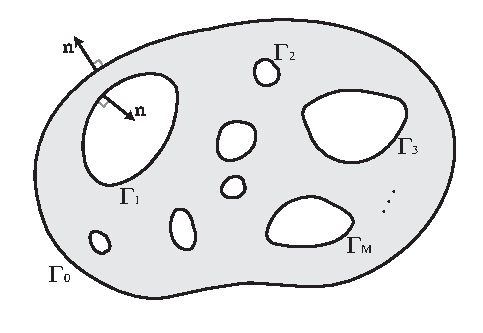
\includegraphics[height=2in]{fig1.eps}
\end{array}$
  \caption{\em A  bounded multiply-connected domain $D$.  The outer 
    boundary is denoted by $\Gamma_0$ (which is absent in unbounded domains) and the interior component 
    curves by $\Gamma_1,\cdots,\Gamma_M$. The unit normal $\n$ points out of $D$ on each component curve.}
  \label{fig1}
\end{figure}

\section{Potential theory and integral equation formulations}
To fix
notation, let us consider a domain $D$ with boundary $\Gamma$
which is $M$ or $(M+1)$-ply connected (\Figr{fig1}).
We are interested in solving\eqr{eq:mod_lap_hom}, subject to both Dirichlet and Neumann boundary conditions. 
In both cases, we start with the free-space Green's function $G(\y - \x) =
G(y_1- x_1, y_2-x_2)$ for the operator $1-\alpha^2\Delta$, 
\[
  G(\x) = \frac{1}{2\pi\alpha^2} K_0 \left( \frac{|\x|}{\alpha} \right) ,
\]
where $K_0$ is the zeroth-order modified Bessel's function of the second
kind.
The Dirichlet problem is considered in section 2.1 and the Neumann problem in 2.2.

\subsection{The Dirichlet Problem}
Consider the following Dirichlet problem:
\begin{eqnarray}
  u(\x) - \alpha^2 \Delta u(\x) = 0, && {\x} \in D,  \nonumber \\
  u(\x) = f(\x), && \x \in \Gamma.
  \label{dirichlet:bc}
\end{eqnarray}
If $D$ is unbounded, the appropriate decay
conditions for the solution is $u(\x) \rightarrow 0$ as $|\x|
\rightarrow \infty$.
We seek the solution $u(\x)$ in the form of a double layer potential, 
\begin{equation}
  u(\x)=\frac{1}{2\pi\alpha^2}\int_{\Gamma}\pderiv{}{n_{\y}}K_{0}
  \left(\frac{|\y-\x|}{\alpha} \right) \sigma(\y) \, ds_{\y}, \qquad \x \in D, 
  \label{eq:u_dirichlet}
\end{equation}
where $\sigma(\y)$ is the value of the unknown
density at the boundary point $\y$, and $\partial / \partial n_\y$
represents the outward normal derivative at the point $\y$.

In order to derive the form of the integral equation based on the representation\eqr{eq:u_dirichlet}, we must understand the behaviour of the potential on the boundary $\Gamma$. 
We note that as $z \rightarrow 0$, 
\[
 K_0 (z) \sim -\log(z) + Q(z), 
\]
where $Q(z)$ is a polynomial in $z$ \cite{ABRAM}. 
Thus,\eqr{eq:u_dirichlet} behaves asymptotically as if it has a logarithmic kernel, and we note for future reference that 
\begin{equation}
  \lim_{\tiny{\begin{array}{r}\y \rightarrow \x \smallskip \label{jump2} \\
        \x, \y \in \Gamma
      \end{array} }}
  \pderiv{}{n_{\y}}K_{0}\left(\frac{|\y-\x|}{\alpha}\right) = 
  -\frac{1}{2}\kappa(\x),
\end{equation}
where $\kappa(\x)$ denotes the curvature of $\Gamma$ at the point
$\x$.

The jump relations for potentials of the logarithmic kernel are well known, and therefore,  for  any point $\x$ on the boundary $\Gamma$,
\begin{eqnarray*}
  \lim_{\tiny{\begin{array}{l}
        \x'  \rightarrow \x  \\
        \x'  \in  D 
      \end{array} }}
  u(\x')& = &  
  -\frac{1}{2\alpha^2}\sigma(\x)+\frac{1}{2\pi\alpha^2}\int_{\Gamma}
  \pderiv{}{n_{\y}}K_{0}\left(\frac{|\y-\x|}{\alpha}\right)
  \sigma(\y)\, ds_{\y}, \\
  \lim_{\tiny{\begin{array}{l}
        \x'  \rightarrow  \x \\
        \x'  \in  D^c 
      \end{array} }}
  u(\x')& = &  \frac{1}{2\alpha^2}\sigma(\x)+
  \frac{1}{2\pi\alpha^2}\int_{\Gamma}\pderiv{}{n_{\y}}
  K_{0}\left(\frac{|\y-\x|}{\alpha}\right)\sigma(\y)\, ds_{\y}.
\end{eqnarray*}
Using the first limit in the preceding expression, and matching to the boundary condition\eqr{dirichlet:bc}, we obtain an integral equation for the layer density $\sigma$:
\begin{equation}
  \label{dirichlet:inteqn}
\sigma(\x)- \frac{1}{\pi}
  \int_{\Gamma}\pderiv{}{n_{\y}}K_{0}\left(\frac{|\y - \x|}{\alpha}\right)
  \sigma(\y)\, ds_{\y} = -2 \alpha^2 f(\x) .
\end{equation}

\subsection{The Neumann Problem}
Consider the following Neumann problem:
\begin{eqnarray*}
  u(\x) - \alpha^2 \Delta u(\x) = 0, &&{\x} \in D, \\
  \frac{\partial u(\x)}{\partial n} = g(\x), && \x \in \Gamma.
\end{eqnarray*}
We seek the solution $u(\x)$ in the form of a single layer potential
\begin{align*}
  u(\x)=\frac{1}{2\pi\alpha^2}\int_{\Gamma} K_{0}
  \left(\frac{|\y-\x|}{\alpha} \right) \sigma(\y) \, ds_{\y}.
\end{align*}
In order to satisfy the boundary conditions, the density
$\sigma(\x)$ must satisfy the integral equation
\begin{equation}
  \label{neumann:inteqn}
 \sigma(\x) + \frac{1}{\pi}
  \int_{\Gamma}\pderiv{}{n_{\x}}K_{0}\left(\frac{|\y - \x|}{\alpha}
  \right)\sigma(\y)ds_{\y}= 2\alpha^2 g(\x) .
\end{equation}
We note that from\eqr{jump2}, the kernels in the integral equations\eqr{dirichlet:inteqn} and\eqr{neumann:inteqn} are bounded and continuous along
$\Gamma$, and thus the integral operators are compact.
In addition, there are no nontrivial
homogeneous solutions. Therefore, by the Fredholm alternative,
\eqr{dirichlet:inteqn} and\eqr{neumann:inteqn} have unique solutions for any integrable data
$f(\x)$ or $g(\x)$.

In summary, equations\eqr{dirichlet:inteqn} and\eqr{neumann:inteqn} can be
written in the general form:
\begin{equation}
   \sigma(\x) + \frac{1}{\pi} \int_{\Gamma} K(\y,\x) \sigma(\y) \, ds_{\y} = F(\x). 
\label{gen_int_eqn}
\end{equation}
In the case of the Dirichlet problem, we have
\[
   \begin{array}{rcl}
      K(\y,\x) & = & \displaystyle{\frac{1}{\alpha} K_1 \left( \frac{|\y - \x|}{\alpha} \right)
                         \frac{\y-\x }{|\y - \x|} \cdot {\bf n}_{\y}, }  \smallskip \\
             F(\x) & = & -2\alpha^2 f(\x) .
   \end{array}
\]
In the case of the Neumann problem, we have 
\[
    \begin{array}{rcl}
      K(\y,\x) & = & \displaystyle{\frac{1}{\alpha} K_1 \left( \frac{|\y - \x|}{\alpha} \right)
                         \frac{\y-\x }{|\y - \x|} \cdot {\bf n}_{\x}, }   \smallskip \\
      F(\x) & = & 2\alpha^2 g(\x) .
    \end{array}
\]

\section{Numerical methods}
We assume each component curve $\Gamma_k$, $k=1,\cdots, M$, is
parametrized by $\y^k(\alpha)$, where $\alpha \in [0, 2\pi)$. Similarly, $\sigma^k(\alpha)$ refers to the restriction of the density $\sigma$ on $\Gamma_k$.
On each
contour $\Gamma_k$, we are given $N$ points equispaced with respect
to $\alpha$. Thus the mesh spacing is $h = 2\pi/N$, and the total
number of discretization points is $N M$. Associated with each
such point, denoted by $\y^k_j$, is an unknown density $\sigma^k_j$.

The presence of the logarithmic singularity in the integral operator causes the spectrum of kernels based on the Yukawa potential to decay slowly. 
Applying the straightforward
Nystr\"{o}m discretization based on the trapezoidal rule would result in a significant loss of accuracy.
Instead, we use 
hybrid gauss-trapezoidal quadrature rules developed by Alpert \cite{alpert:quad:rules} which are tailored for integrands with logarithmic singularities. 
These quadratures are of order $h^p \log h$. The order $p$ determines a set of nodes $v_n$ and weights  $u_n$, $n=1, \cdots,  l$.
These nodes and weights are used for the quadrature within the interval $\alpha \in [\alpha_j- h a, \alpha_j+h a]$, on $\Gamma_k$ ($a$ and $l$ are also determined by $p$). 
Outside of this interval, the trapezoid rule is used.
Applying this quadrature to\eqr{gen_int_eqn} yields
\begin{align}
    \sigma_j^k & + \frac{h}{\pi} \left\{
    \sum_{\tiny{\begin{array}{l}
                             m=0  \\
                            m \ne k
                 \end{array} }
                }^M  \sum_{n=1}^{N} K(\y^m_n,\y^k_j)\, |\w^m_n| \, \sigma^m_n 
    + \sum_{n=j+a}^{N + j-a} K(\y^k_n,\y^k_j)\, |\w^k_n| \, \sigma^k_n  \right\}  
                         \nonumber \\
    &   + \frac{1}{\pi} \sum_{\tiny{ \begin{array}{l}
                             n=-l  \\
                            n \ne 0
                         \end{array} }}^l \, u_{|n|} 
             K(\y^k_{j + \frac{ n}{|n|} v_{|n|}}, \y^k_j ) 
            \, |\w^k_{j + \frac{ n}{|n|} v_{|n|}  } | \, \sigma^k_{j + \frac{n}{|n|} v_{|n|}} 
             =  F_j^k.          
             \label{discrete_sys}
\end{align}
In the second sum, we invoke periodicity of all functions on $\Gamma_k$, or equivalently, $j+N_k = j$. In the final sum, we are required to know values of $\sigma$ intermediate to the nodal values at $\alpha=\alpha_j \pm h v_{|n|}$. 
In these cases, we use Fourier interpolation (this increases the computational complexity to $O(N\log N)$; however other interpolation methods that are less expensive, but also less accurate, could be used).

Equation\eqr{discrete_sys} is a dense $MN\times MN$ linear system that must be solved for the unknowns $\sigma_j^k$. 
In our implementation,\eqr{discrete_sys} is solved iteratively, using GMRES \cite{SAAD}. 
The bulk of the work at each iteration lies in applying the linear system to a vector. 
Done directly, this would require $O(N^2 M^2)$ operations for each iteration. 
This cost can be reduced to $O(NM)$ by using the adaptive fast multipole method, the details of which are outlined in the next section.

Since the number of iterations needed to solve a Fredholm equation of the second kind to a fixed precision is bounded independent of the system size $N$ (holding the geometry fixed), the total number of operations required to solve\eqr{discrete_sys} is $O(NM)$. 

\section{The fast multipole method}
Consider a collection of $N$ particles or ``sources'' in $\RR^{2}$, $\x_1$, $\x_2$, $\cdots$, $\x_{N}$, together with corresponding source strengths $q_1$, $q_2$, $\cdots$, $q_{N}$. 
We are interested in efficiently evaluating the following:
\begin{equation}
     \Phi(\x_j)=\sum^{N}_{\tiny \begin{array}{ll}
                                     i=1 \vspace{-.01in} \\
                                     i\ne j
                                  \end{array}
                                }
    q_{i} \, K_{0}\left(\frac{|\x_{j}-\x_i|}{\alpha}\right), \qquad j = 1, \cdots, N. 
    \label{direct_potential}
 \end{equation}

The fast multipole method was developed to evaluate fields based on the Coulomb potential in two dimensions \cite{CGR,fmm}. 
The FMM has since been extended to include other potential functions, such as the three-dimensional Yukawa potential \cite{screened_coulomb}. 
An FMM developed to evaluate volume potentials based on the two-dimensional Yukawa potential appears in \cite{modified:helmholtz}; we use this work as the basis for our ``particle-to-particle'' FMM required to evaluate\eqr{discrete_sys}. 
Our FMM is identical in structure to the one presented in \cite{modified:helmholtz}, with only minor modification. 
For more detail, we refer the reader to this work and others \cite{screened_coulomb,new_FMM} which discusses the use of exponential expansions. 
Here, we present a minimal sketch of the FMM algorithm as it applies to our problem at hand. 

The FMM uses an adaptive quad-tree structure in order to superimpose a hierarchy of refinements on the computational domain.
We imbed the geometry inside a unit square $S$, which is considered to be grid level 0.
Grid level $l+1$ is obtained recursively by subdividing each square $s$ at level $l$ into four equal parts, which are the ``children'' of $s$. 
Adaptivity is achieved by not requiring the same number of levels of subdivision in all regions of $S$. 
The basic idea of the FMM is that for each particle, contributions from ``nearby'' (neighbour) particles to the potential field are handled directly via\eqr{direct_potential}, while ``far-field'' (non-neighbour) interactions are handled using multipole and/or related expansions. 

The first step in the FMM is to form the multipole expansions for all of the nodes (boxes) in the quad-tree structure. 
The following theorem follows from Graf's addition theorem, and corresponds to Theorem 3 in \cite{modified:helmholtz} with modifications made for particle to particle interactions:
\begin{theorem}[Multipole Expansion]
  Let $s$ be a node in the quad-tree centred at $\s=(s_1,s_2)$. 
  Assume $s$ is not a neighbour of $B$.
  Then the potential $\Phi(\x)$ due to $s$ for $\x \in B$ is given by the multipole expansion
  \[
     \Phi(\x) = \sum_{\x_{i} \in B} q_{i} K_{0}
  \left(\frac{|\x-\x_{i}|}{\alpha}\right)
   = \sum_{l=-\infty}^{\infty} M_l K_l \left( \frac{|\x-\s|}{\alpha}  \right) e^{i l \theta_\x},
  \]
  where
  \[
   M_{l} = \sum_{\x_{i} \in B} q_{i}
                I_{l}\left( \frac{|\x_{i} - \s|}{\alpha}
                             \right)e^{-i l \theta_{\x_{i}}}.
  \]
Here, $I_l$ and $K_l$ are the $l^{th}$ order modified Bessel's function of the first and second kind, respectively, and $\theta_\x$ and $\theta_{\x_{i}}$ denote the polar angles for $\x$ and $\x_i$ with respect to $\s$.
\end{theorem}

The second step of the FMM is to construct a  {\em local expansion} for each node $B$. In order to translate the multipole expansions to local ones, we apply the following result:
\begin{theorem}[Local Expansion]
 Suppose a multipole expansion associated with node $s$ centred at $\s$ is given by
  \[
     \Phi(\x) 
   = \sum_{n=-\infty}^{\infty} M_n K_n \left( \frac{|\x-\s|}{\alpha}  \right) e^{i l \theta_\x}.
  \]
 Further assume $s$ is in the ``far field'' of $B$.
 Then for any $\x \in B$, $\Phi(\x)$ can be represented as a local expansion
\[
   \Phi(\x) =  \sum_{l=-\infty}^{\infty} L_l I_l \left( \frac{\rho}{\alpha}  \right) e^{i l \theta},
\]
where $(\rho,\theta)$ denote the polar coordinates of $\x$ with respect to the centre of $B$, and the local coefficients are expressed using the ``multipole to local'' translation operator defined by 
  \[
  L_{l} = \sum_{n=-\infty}^\infty
                M_n K_{l-n}\left( \frac{\rho_0}{\alpha}
                             \right)e^{-i (l-n) \theta_0 }.
  \]
Here, $(\rho_0,\theta_0)$ are the polar coordinates of the centre of $B$ with respect to $\s$.
\end{theorem}

The work required in the above Theorem represents the bulk of the operation count in the FMM. 
This work can be significantly reduced by using plane wave representations and a ``diagonal translation operator'' (c.f. Appendices A and C in \cite{modified:helmholtz}). 
The savings in cost are shown in \tabr{table1}.
The rest of the original FMM procedure proceeds as in sections 2 and 3 in \cite{modified:helmholtz}, and we will not elaborate further.  

\begin{table}[htbp]
\begin{center}
\begin{tabular*}{\textwidth}{@{\extracolsep{\fill}}rccc}     \hline
\multicolumn{1}{c}{$N$} & Direct & Original FMM & Plane-Wave FMM  \\ \hline
64    &  0.01 & 0.06             & 0.06 \\  
128   & 0.03 & 0.08             & 0.08 \\  
256   & 0.08 & 0.22             &  0.12 \\  
512   & 0.30 & 0.47             & 0.21 \\  
1024   & 1.15 & 1.03           & 0.36 \\ 
2048   & 4.59 & 2.02           & 0.60 \\ 
4096   & 18.26 & 3.86         & 1.36 \\ 
8192   & 73.42 & 9.46         & 2.02 \\ 
16384   & 292.52 & 14.80   & 4.60 \\ 
32768   & 1168.22 & 38.44 & 7.04 \\ 
65536  & 4689.96 & 56.55  &  17.42   \\ \hline
\end{tabular*}
\end{center}
\caption{A comparison of the CPU time (in seconds) required to compute the potential due to a set of points directly, via the original FMM based on multipole to local translations, or via the FMM based on plane-wave expansions.
Half of the points are randomly placed in the unit square 
and the other half are concentrated on two elliptical boundaries.
\label{table1} }
\end{table}

Evaluating\eqr{discrete_sys}, however, is not as simple as calculating a sum in the form of\eqr{direct_potential}.
In the case of the Neumann problem, we are required to evaluate a potential of the form 
\begin{eqnarray*}
     \frac{\partial \Phi \,}{\partial n_{\x_j}} (\x_j) & = & \sum_{\small  i\ne j }
    q_{i} \, \nabla_{\x_{j}} K_{0}\left(\frac{|\x_{j}-\x_i |}{\alpha}\right) \cdot \n_j  \\
                         & = & \nabla_{\x_{j}} \Phi(\x_j) \cdot \n_j \, . 
 \end{eqnarray*}
This evaluation is relatively straightforward as $\nabla_{\x_{j}} \Phi ({\x_{j}})$ relies on the same multipole coefficients as $\Phi ({\x_{j}})$.
In the case of the Dirichlet problem, we are required to evaluate a potential of the form
\begin{equation*}
     \frac{\partial \Phi \,}{\partial n_{\x_i}} (\x_j) =\sum_{\small  i\ne j }
    q_{i} \, \nabla_{\x_{i}} K_{0}\left(\frac{|\x_{j}-\x_i |}{\alpha}\right) \cdot \n_i \, .  
 \end{equation*}
In this case, the multipole coefficients do change:
\[
   M_{l} = \sum_{\x_{i} \in B} q_{i}
                \frac{\partial \,}{\partial n_{\x_i}} I_{l}\left( \frac{|\x_{i} - \s|}{\alpha}
                             \right)e^{-i l \theta_{\x_{i}}}.
\]

%%%%%%%%%%%%%%%%%%%%%%%%%%
\begin{figure}[htps]
     \centering
$\begin{array}{c}
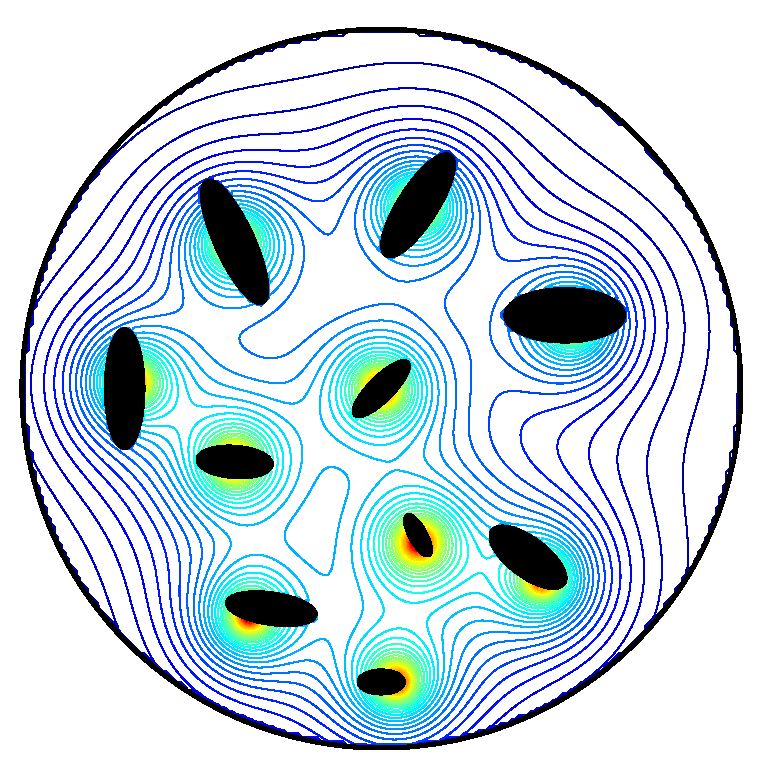
\includegraphics[height=2in]{figure2.eps} 
\end{array}$
  \caption{\em The solution to Example 1.}
  \label{fig2}
\end{figure}
\section{Numerical Results}
The algorithms described above have been implemented in Fortran. The tolerance for convergence of GMRES is set to $10^{-11}$. 
Here, we illustrate the performance on a variety of examples.
All timings cited are for a single processor on a Mac Pro 2.1 with two 3GHz Quad-Core Intel Xeon processors.

\noindent {\bf Example 1:} We first consider the problem of solving\eqr{eq:mod_lap_hom} with $\alpha=0.1$ in a bounded, circular domain with ten interior elliptic contours (see \figr{fig2}). 
We generate the Dirichlet boundary conditions from
\begin{equation}
   u(\x) = \sum_{k=1}^{10}K_0 \left( \frac{|\x - \x_k |}{\alpha} \right),
   \label{exact_sol}
\end{equation}
where $\x_k$ is a point inside $\Gamma_k$.
We test the performance of our methods using quadrature rules of varying degree of accuracy. 
The results are shown in \tabr{table2} through \tabr{table6}. 
These tables confirm that the number of GMRES iterations required for convergence is independent of $N$. 
Also, we see near-linear scaling of the CPU time with $N$. 
In terms of overall accuracy, we see the best overall performance with the $O(h^8 \log h)$ scheme.

\begin{table}[htbp]
\begin{center}
\begin{tabular*}{\textwidth}{@{\extracolsep{\fill}}rccl}     \hline
\multicolumn{1}{c}{$N$} & \multicolumn{1}{c}{\# Iterations} 
& \multicolumn{1}{c}{CPU Time} 
& \multicolumn{1}{c}{Error} \\ \hline
704    &  45 & 12.1 & $3.80 \, 10^{-6}$ \\  
1408   & 45 & 20.3 & $3.36 \, 10^{-7}$ \\  
2816   & 45 & 40.1 &  $4.20 \, 10^{-8}$ \\  
5632   & 45 & 83.9 & $5.25 \, 10^{-9}$  \\  \hline
%11264   & 45 & 147.8 & $7.72 \, 10^{-10}$ \\  \hline
\end{tabular*}
\end{center}
\caption{Performance of the algorithm on example 1. Trapezoid Rule. CPU time is measured in seconds. 
\label{table2} }
\end{table}
%%%%
\begin{table}[htbp]
\begin{center}
\begin{tabular*}{\textwidth}{@{\extracolsep{\fill}}rccl}     \hline
\multicolumn{1}{c}{$N$} & \multicolumn{1}{c}{\# Iterations} 
& \multicolumn{1}{c}{CPU Time} 
& \multicolumn{1}{c}{Error} \\ \hline
704    &  45 & 12.3 & $9.95 \, 10^{-7}$ \\  
1408   & 45 & 20.2 & $3.60 \, 10^{-7}$ \\  
2816   & 45 & 41.1 &  $5.71 \, 10^{-8}$ \\  
5632   & 45 & 87.7 & $8.65 \, 10^{-9}$  \\  \hline
%11264   & 45 & 150.1 & $1.49 \, 10^{-9}$ \\  \hline
\end{tabular*}
\end{center}
\caption{Performance of the algorithm on example 1. Quadrature is $O(h^2 \log h)$. CPU time is measured in seconds.
\label{table3} }
\end{table}
%%%%
\begin{table}[htbp]
\begin{center}
\begin{tabular*}{\textwidth}{@{\extracolsep{\fill}}rccl}     \hline
\multicolumn{1}{c}{$N$} & \multicolumn{1}{c}{\# Iterations} 
& \multicolumn{1}{c}{CPU Time} 
& \multicolumn{1}{c}{Error} \\ \hline
704    &  45 & 12.5 & $1.11 \, 10^{-6}$ \\  
1408   & 45 & 21.1 & $4.92 \, 10^{-10}$ \\  
2816   & 45 & 42.3 &  $3.19 \, 10^{-12}$ \\  
5632   & 45 & 88.9 & $2.26 \, 10^{-13}$  \\  \hline
%11264   & 45 & 158.47 & $1.57 \, 10^{-12}$ \\  \hline
\end{tabular*}
\end{center}
\caption{Performance of the algorithm on example 1. Quadrature is $O(h^4 \log h)$. CPU time is measured in seconds.
\label{table4} }
\end{table}
%%%%
\begin{table}[htbp]
\begin{center}
\begin{tabular*}{\textwidth}{@{\extracolsep{\fill}}rccl}     \hline
\multicolumn{1}{c}{$N$} & \multicolumn{1}{c}{\# Iterations} 
& \multicolumn{1}{c}{CPU Time} 
& \multicolumn{1}{c}{Error} \\ \hline
704    &  45 & 13.3 & $1.11 \, 10^{-6}$ \\  
1408   & 45 & 22.5 & $5.41 \, 10^{-10}$ \\  
2816   & 45 & 45.0 &  $5.88 \, 10^{-13}$ \\  
5632   & 45 & 94.2 & $8.55 \, 10^{-14}$  \\  \hline 
%11264   & 45 & 168.0 & $1.14 \, 10^{-11}$ \\  \hline
\end{tabular*}
\end{center}
\caption{Performance of the algorithm on example 1. Quadrature is $O(h^8 \log h)$. CPU time is measured in seconds.
\label{table5} }
\end{table}
%%%%
\begin{table}[htbp]
\begin{center}
\begin{tabular*}{\textwidth}{@{\extracolsep{\fill}}rccl}     \hline
\multicolumn{1}{c}{$N$} & \multicolumn{1}{c}{\# Iterations} 
& \multicolumn{1}{c}{CPU Time} 
& \multicolumn{1}{c}{Error} \\ \hline
704    &  45 & 14.7 & $1.11 \, 10^{-6}$ \\  
1408   & 45 & 25.2 & $5.50 \, 10^{-10}$ \\  
2816   & 45 & 50.2 &  $1.40 \, 10^{-11}$ \\  
5632   & 45 & 104.5 & $1.44 \, 10^{-11}$   \\  \hline
%11264   & 45 & 168.0 & $1.14 \, 10^{-11}$ \\  \hline
\end{tabular*}
\end{center}
\caption{Performance of the algorithm on example 1. Quadrature is $O(h^{16} \log h)$. CPU time is measured in seconds.
\label{table6} }
\end{table}

%%%%
\noindent {\bf Example 2:} We now consider an exterior Neumann problem, whose boundary conditions are, again, derived from\eqr{exact_sol}. 
The geometry is also the same as in the preceding example, minus the outer boundary. 
Based on previous results, we select the $O(h^8\log h)$ quadrature rule, and we examine the performance of the methods for different values of $\alpha$ in\eqr{eq:mod_lap_hom}.
The results are shown in \tabr{table7} through \tabr{table16}. 
Interestingly enough, the conditioning of the linear system appears relatively independent of $\alpha$ for $\alpha > 0.1$. 
This is not the case for the Dirichlet problem, where we observed that the number of GMRES iterations visibly increases as $\alpha$ increases in size. 
This is to be expected, as the governing equation becomes more harmonic, and the integral equation based on the double layer potential for Laplace's equation in multiply connected domains is known to become rank deficient \cite{mult:conn}.
Since we are anticipating applications in which $\alpha$ is proportional to a time step, we are not concerned here with this behaviour.
%%%%  alpha = 10.0
\begin{table}[htbp]
\begin{center}
\begin{tabular*}{\textwidth}{@{\extracolsep{\fill}}rccl}     \hline
\multicolumn{1}{c}{$N$} & \multicolumn{1}{c}{\# Iterations} 
& \multicolumn{1}{c}{CPU Time} 
& \multicolumn{1}{c}{Error} \\ \hline
704    &  23 & 4.3 & $1.99 \, 10^{-6}$ \\  
1408   & 23 & 6.8 & $2.08 \, 10^{-11}$ \\  
2816   & 23 & 13.5 &  $1.71 \, 10^{-13}$ \\  
5632   & 23 & 26.7 & $1.81 \, 10^{-13}$    \\  \hline 
\end{tabular*}
\end{center}
\caption{Performance of the algorithm on example 2 with $\alpha = 10$. CPU time is measured in seconds.
\label{table7} }
\end{table}
%%%%    alpha = 1.0
\begin{table}[htbp]
\begin{center}
\begin{tabular*}{\textwidth}{@{\extracolsep{\fill}}rccl}     \hline
\multicolumn{1}{c}{$N$} & \multicolumn{1}{c}{\# Iterations} 
& \multicolumn{1}{c}{CPU Time} 
& \multicolumn{1}{c}{Error} \\ \hline
704    &  23 & 4.5 & $1.83 \, 10^{-6}$ \\  
1408   & 23 & 6.9 & $1.87 \, 10^{-11}$ \\  
2816   & 23 & 13.7 &  $4.37 \, 10^{-13}$ \\  
5632   & 23 & 26.7 & $6.33 \, 10^{-13}$    \\  \hline 
\end{tabular*}
\end{center}
\caption{Performance of the algorithm on example 2 with $\alpha = 1$. CPU time is measured in seconds.
\label{table10} }
\end{table}
%%%%    alpha = 0.1
\begin{table}[htbp]
\begin{center}
\begin{tabular*}{\textwidth}{@{\extracolsep{\fill}}rcrl}     \hline
$N$ & \# Iterations & CPU Time & Error \\ \hline
704    &  25 & 6.5 & $5.43 \, 10^{-7}$ \\  
1408   & 25 & 8.8 & $6.91 \, 10^{-12}$ \\  
2816   & 25 & 16.4 &  $4.67 \, 10^{-12}$ \\  
5632   & 25 & 31.6 & $4.21 \, 10^{-12}$    \\  \hline 
\end{tabular*}
\end{center}
\caption{Performance of the algorithm on example 2 with $\alpha = 0.1$.  CPU time is measured in seconds.
\label{table13} }
\end{table}
%%%%    alpha = 0.01
\begin{table}[htbp]
\begin{center}
\begin{tabular*}{\textwidth}{@{\extracolsep{\fill}}rccl}     \hline
\multicolumn{1}{c}{$N$} & \multicolumn{1}{c}{\# Iterations} 
& \multicolumn{1}{c}{CPU Time} 
& \multicolumn{1}{c}{Error} \\ \hline
704    &  15 & 3.6 & $6.33 \, 10^{-11}$ \\  
1408   & 15 & 6.9 & $6.91 \, 10^{-11}$ \\  
2816   & 15 & 14.5 &  $2.77 \, 10^{-12}$ \\  
5632   & 15 & 27.0 & $6.45 \, 10^{-12}$     \\  \hline
\end{tabular*}
\end{center}
\caption{Performance of the algorithm on example 2 with $\alpha = 0.01$. CPU time is measured in seconds.
\label{table16} }
\end{table}

\begin{figure}[htps]
     \centering
$\begin{array}{cc}
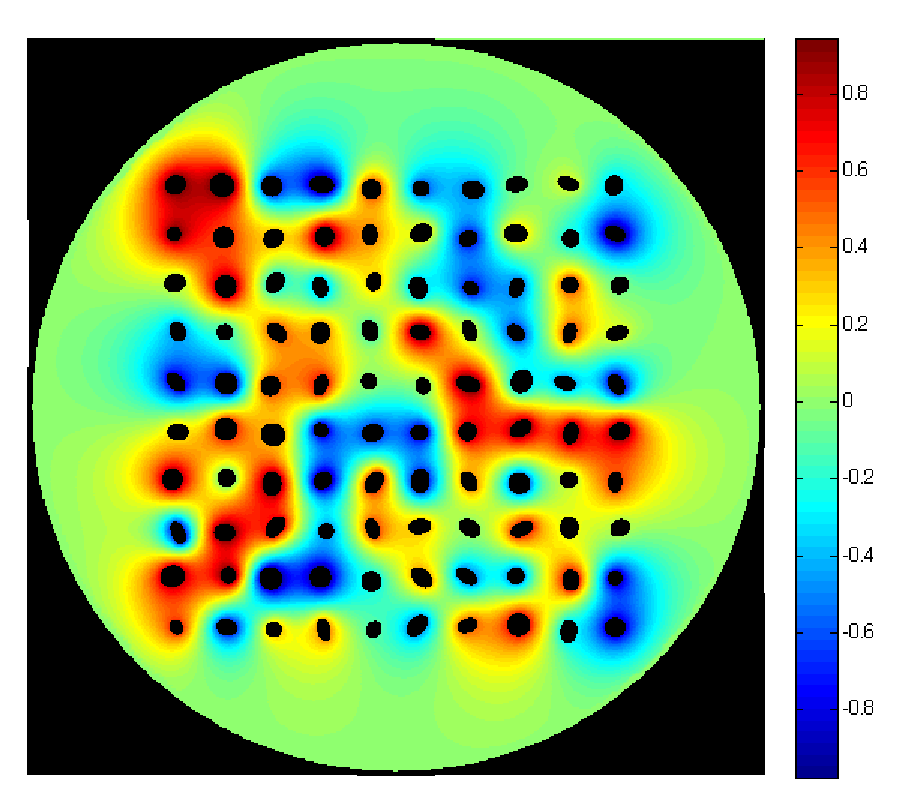
\includegraphics[height=2in]{figure3_a.eps} &
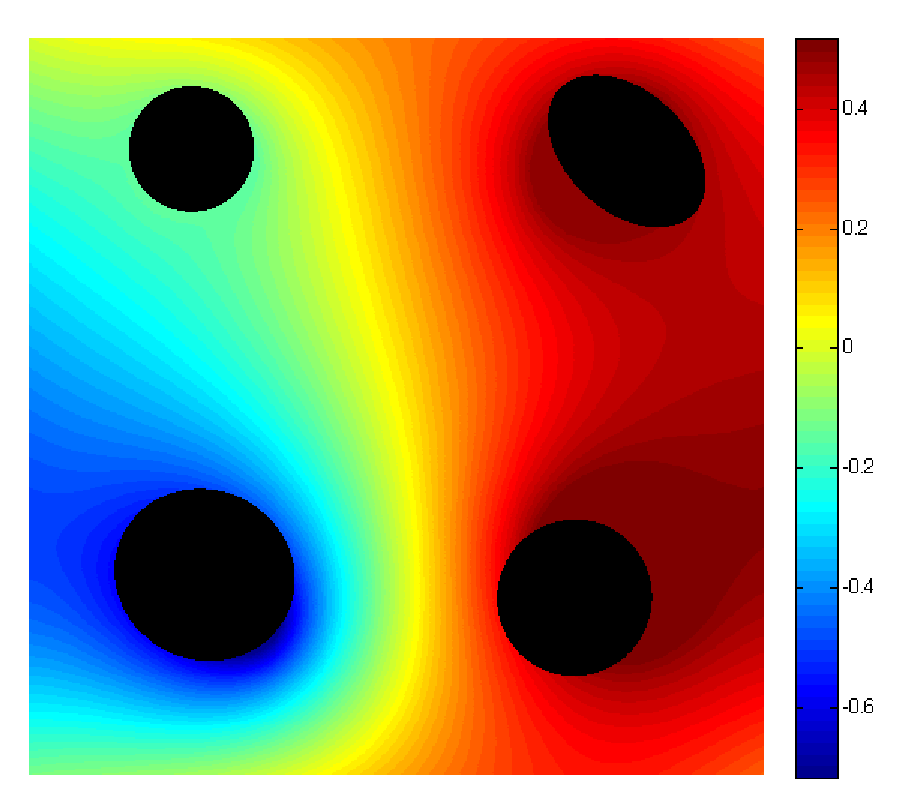
\includegraphics[height=2in]{figure3_b.eps}
\end{array}$
  \caption{\em The solution to example 3. There are 512 points per hole, $N=51712$, 88 GMRES iterations are required, consuming 1510.7 $s$ of CPU time. The plot on the right shows a close-up of the solution from a small region from the upper left quadrant of the domain.}
  \label{figure3}
\end{figure}
\noindent {\bf Example 3:} We next consider a larger-scale problem. We compute the solution to the modified Helmholtz equation with $\alpha=0.1$ in a bounded domain with $100$ elliptical contours that have varying proportions and alignment (\figr{figure3}). On each of these contours, we prescribe a constant Dirichlet boundary conditions selected randomly from $(-1,1)$. Each contour is discretized with $512$ points, resulting in a matrix of order 51712. 
The total CPU time to solve this linear system to a tolerance of $10^{-11}$ required approximately 25 minutes. 

\begin{figure}[htps]
     \centering
$\begin{array}{c}
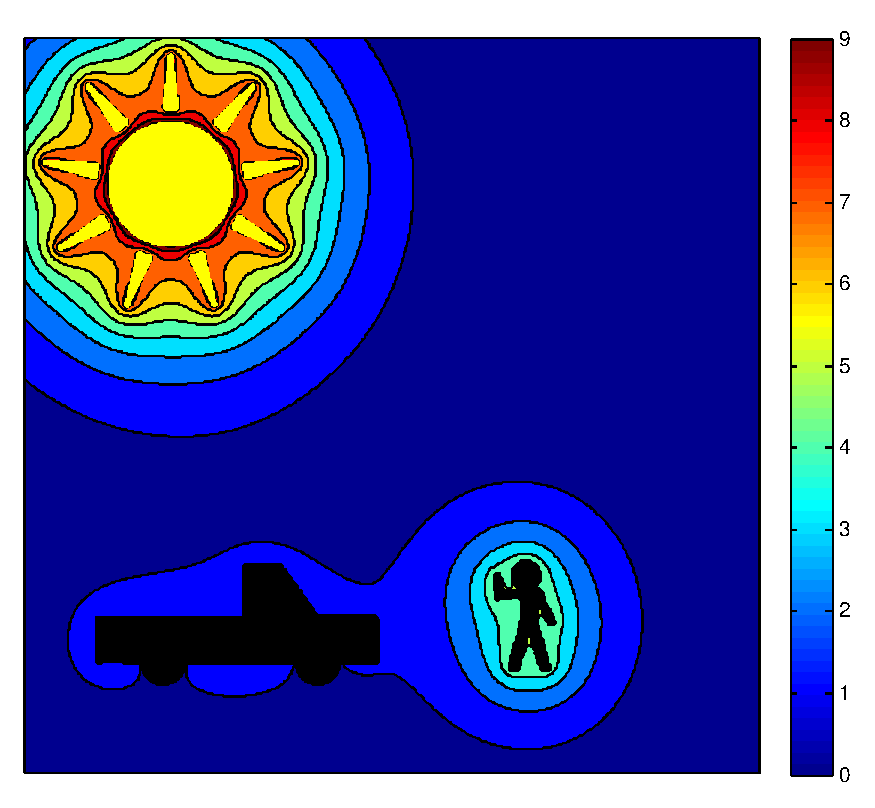
\includegraphics[height=3in]{figure4.eps} 
\end{array}$
  \caption{\em The solution to example 4 with N=30,560.  67 GMRES iterations are required, requiring 361.5 $s$ of CPU time.}
  \label{figure4}
\end{figure}
\noindent {\bf Example 4:} While the domains in the preceding examples are multiply connected, the individual contours have consisted of rather simple shapes. In this example, we consider more complex contours (\figr{figure4}). 
We solve equation\eqr{eq:mod_lap_hom} in an unbounded domain with $\alpha = 0.1$. Dirichlet boundary conditions are assigned in the following way: we assign a value of 1 on the wheels of the truck, a value of 2 to the rest of the truck, a value of 5 on the man, and 10 to the sun and its rays.
%%%%%%%%%%%%%%%%%%%%%%%%%%
%\begin{center}
\section{Conclusions}
We have presented a class of integral equation methods for the solution to the modified Helmholtz equation in bounded or unbounded multiply-connected domains. 
Using a fast-multipole accelerated iterative method, our solution procedure requires $O(N)$ operations, where $N$ is the number of nodes in the discretization of the boundary. 
With these techniques, and using only modest computational resources, we were able to accurately and efficiently solve problems in highly complex domains.
We believe we have demonstrated that these methods have the potential to be highly suitable for solving large-scale problems.

The immediate focus of future work is to develop integral equation techniques to solve\eqr{eq:mod_lap_inhom} in arbitrary geometry.  To do this, we must couple our solver with the solver presented in \cite{modified:helmholtz}. 
Once that is achieved, we will apply these integral equation techniques to solve the equations that arise from the temporal discretization of convection-diffusion type equations.
In this way, we hope to demonstrate that integral equation methods offer an attractive alternative to conventional finite element and finite difference methods for many large-scale problems from engineering and physics.

%\end{center}

\begin{thebibliography}{10}

\bibitem{ABRAM}
M.~Abramowitz and I.A. Stegun, editors.
\newblock {\em {Handbook of Mathematical Functions}}.
\newblock Dover, New York, NY, 1964.

\bibitem{alpert:quad:rules}
B.~Alpert.
\newblock {Hybrid Gauss-Trapezoidal Quadrature Rules}.
\newblock {\em SIAM Journal of Scientific Computing}, 20:1551--1584, 1999.

\bibitem{CGR}
J.~Carrier, L.~Greengard, and V.~Rokhlin.
\newblock A fast adaptive multipole algorithm for particle simulations.
\newblock {\em SIAM J. Sci. Statist. Comput.}, 9:669--686, 1988.

\bibitem{modified:helmholtz}
H.~Cheng, J.~Huang, and Leiterman T.
\newblock {An Adaptive Fast Solver for the Modified Helmholtz Equation in Two
  Dimensions}.
\newblock {\em J. Comp. Phys.}, 211:616--637, 2006.

\bibitem{mult:conn}
L.~Greenbaum, A.~Greengard and G.B. McFadden.
\newblock {Laplace's Equation and the Dirichlet-Neumann Map in Multiply
  Connected Domains}.
\newblock {\em J. Comp. Phys.}, 105:267--278, 1993.

\bibitem{screened_coulomb}
L.~Greengard and J.~Huang.
\newblock {A new version of the fast multipole method for screened Coulomb
  interactions in three dimensions}.
\newblock {\em J. Comp. Phys.}, 180:642--658, 2002.

\bibitem{int:equation:nse}
L.~Greengard and M.C. Kropinski.
\newblock {An Integral Equation Approach to the Incompressible Navier-Stokes
  Equations in Two Dimensions}.
\newblock {\em SIAM Journal of Scientific Computing}, 20:318--336, 1998.

\bibitem{stokes:flow}
L.~Greengard, M.C. Kropinski, and A.~Mayo.
\newblock {Integral Equation Methods for Stokes Flow and Isotropic Elasticity
  in the Plane}.
\newblock {\em J. Comp. Phys.}, 125:403--414, 1996.

\bibitem{poisson:solver:accuracy}
L.~Greengard and J.-Y. Lee.
\newblock {A Direct Adaptive Poisson Solver of Arbitrary Accuracy}.
\newblock {\em J. Comp. Phys.}, 125:415--424, 1995.

\bibitem{new_FMM}
L.~Greengard and V.~Rokhlin.
\newblock {A new version of the fast multipole method for the Laplace equation
  in three dimensions}.
\newblock {\em Acta Numer.}, 6:229--269, 1997.

\bibitem{fmm}
L.~Greengard and V.~Rokhlin.
\newblock {A Fast Algorithm for Particle Simulations}.
\newblock {\em J. Comp. Phys.}, 73:325--348, 1987.

\bibitem{fast_direct}
Leslie Greengard, Denis Gueyffier, Per-Gunnar Martinsson, and Vladimir Rokhlin.
\newblock Fast direct solvers for integral equations in complex
  three-dimensional domains.
\newblock {\em Acta Numer.}, pages 243--275, 2009.

\bibitem{KUO_et_al}
S.~Kuo, B.~Tidor, and J.~White.
\newblock A meshless, spectrally accurate, integral equation solver for
  molecular surface electrostatics.
\newblock {\em ACM JETC}, 4:353--367, 2008.

\bibitem{Lu_et_al}
B.~Lu, X.~Cheng, J.~Huang, and J.A. McCammon.
\newblock An adaptive fast multipole boundary element method for
  poisson--boltzmann electrostatics.
\newblock {\em J. Chem. Theory and Comp.}, 5:1692--1699, 2009.

\bibitem{Lu_et_al2}
B.Z. Lu, Y.C. Zhou, J.J. Holst, and J.A. McCammon.
\newblock Recent progress in numerical methods for the poisson-boltzmann
  equation in biophysical applications.
\newblock {\em Comm. Comp. Phys.}, 3(5):973--1009, 2008.

\bibitem{martinsson_rokhlin}
P.G. Martinsson and V.~Rokhlin.
\newblock A fast direct solver for boundary integral equations in two
  dimensions.
\newblock {\em J. Comp. Phys.}, 205:1--23, 2005.

\bibitem{nishimura}
N.~Nishimura.
\newblock Fast multipole accelerated boundary integral equation methods.
\newblock {\em Appl. Mech. Rev.}, 55(4):299--324, July 2002.

\bibitem{SAAD}
Y.~Saad and M.H. Schultz.
\newblock Gmres: a generalized minimum residual algorithm for solving
  nonsymmetric linear systems.
\newblock {\em SIAM J. Sci. Stat. Comput.}, 7:856--869, 1986.

\bibitem{ying_biros_zorin}
Lexing Ying, George Biros, and Denis Zorin.
\newblock A high-order 3d boundary integral equation solver for elliptic pdes
  in smooth domains.
\newblock {\em J. Comp. Phys.}, 219:247--275, 2006.

\end{thebibliography}

\end{document}
